\documentclass[10pt]{article}
\usepackage[colorlinks=true,linkcolor=black,urlcolor=black,citecolor=black]%
{hyperref}
\usepackage{proof}
\usepackage{amsmath}
\usepackage{cite}
\usepackage{graphicx}
\usepackage{tikz}
\usepackage{stmaryrd}
\usepackage[normalem]{ulem}
\usetikzlibrary{decorations.markings}
\tikzset{>=latex}

\newcommand\tableflip{
\includegraphics[height=.8\baselineskip]{tableflip.pdf}}
\renewcommand\j{
\includegraphics[height=.6\baselineskip]{j.pdf}\ }
\newcommand\J[1]{\tableflip\rotatebox[origin=c]{180}{#1}}

\newcommand{\msout}[1]{\text{\sout{\ensuremath{#1}}}}
\newcommand\G{\ensuremath{\Gamma}}
\newcommand\type{\ensuremath{\; \mathsf{type}}}
\newcommand\Gpd{\ensuremath{\mathbf{Gpd}}}
\newcommand\Id[3]{\ensuremath{#2 =_{#1} #3}}
\newcommand\interp[1]{\ensuremath{\llbracket #1\rrbracket}}

\newcommand\AccRel{\ensuremath{\overset{?\_?}{\approx}}}
\newcommand\Acc[4]{\ensuremath{#3{:}#1 \AccRel #4{:}#2}}
%TODO a better symbol

\title{The ($\infty$,1)-accidentopos model of\\ unintentional type theory \\
\textsc{\large{(Extended Abstract)}}}
\author{Carlo Angiuli}

\begin{document}
\maketitle

%Weak $\infty$-Groupoid Martin-L\" of type theory

\section{Introduction}

PER Martin-L\"of's intensional type theory (ITT) associates to any elements
$x,y$ of a type $A$ an identity type $\Id Axy$, the type of proofs of equality
of these elements. In \cite{HofmannStreicher}, Hofmann and Streicher showed that
Groupoid Martin-L\"of's ITT can be modeled in the category $\Gpd$, such that any
closed type $A$ is interpreted as a groupoid $\interp{A}$, terms $x,y:A$ are
objects $\interp{x},\interp{y}\in\interp{A}$, and $\interp{\Id Axy}$ is the
discrete groupoid $\hom_{\interp A}(\interp x,\interp y)$.

In general, the identity type itself can have non-trivial morphisms, resulting
in a potentially infinite tower of identity types. This observation has given
rise to semantics in simplicial sets \cite{KapulkinLumsdaineVoevodsky}, or
globular strict \cite{Warren} or weak $\infty$-groupoids.

the Homotopy Type Theory project \cite{HoTT}, 


(More generally, it is
expected that ITT is an internal language for $(\infty,1)$-toposes.)

That such interpretations are possible affords us the
ability to use ITT as a ``natively homotopical'' language for reasoning about
spaces, an idea explored in great detail by \cite{HoTTBook}.

This work focuses on the lesser-known \emph{unintentional type theory} (UTT), a
relative of ITT which has a \emph{mistaken identity} type $\Acc ABxy$, the type
of inadvertent conflations of the terms $x:A$ and $y:B$. This increases the
theory's expressive power by internalizing a type of user error previously
expressible only in meta-metatheory (e.g., blackboards, notes, typesetting, and
so forth).

In particular, we show that UTT is an internal language of
($\infty$,1)-accidentoposes.

%cite Falso

\section{Syntax}

Most of the rules of unintentional type theory are identical to those of
ordinary type theory, as in \cite{Hofmann}. 

\[
\infer[\AccRel F]
  {\G\vdash(\Acc ABMN)\type}
  {\G\vdash M:A & \G\vdash N:B}
\]


\cite{Simmons}

In this way, mistaken 

It is clear that mistaken identities can quickly propagate through

$\msout{asd}$

proof relevant version of \cite{Falso}





The \j rule 
\J{argument}

\section{Semantics}

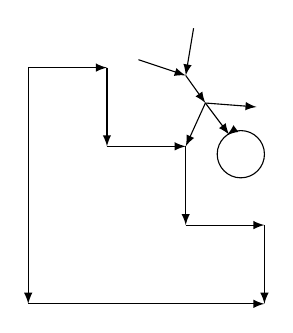
\begin{tikzpicture}
% stairs
\draw[->] (0,3) -- (1,3);
\draw[->] (1,3) -- (1,2);
\draw[->] (1,2) -- (2,2);
\draw[->] (2,2) -- (2,1);
\draw[->] (2,1) -- (3,1);
\draw[->] (3,1) -- (3,0);
\draw[->] (0,3) -- (0,0);
\draw[->] (0,0) -- (3,0);
% head
\draw[decoration={markings, mark=at position 0.35 with {\arrow{>}}},
      postaction={decorate}] (2.7,1.9) circle (0.3);
% torso (2.55,2.15)
\draw[->] (2.25,2.55) -- (2.55,2.15);
\draw[->] (2,2.9) -- (2.25,2.55);
% arms (2.25,2.55)
\draw[->] (2.25,2.55) -- (2.9,2.5);
\draw[->] (2.25,2.55) -- (2.0,2.0);
% legs (2,2.9)
\draw[->] (2.1,3.5) -- (2,2.9);
\draw[->] (1.4,3.1) -- (2,2.9);
\end{tikzpicture}








\pagebreak
\section*{Acknowledgements}

Thanks to Chris Martens for suggesting that I study UTT, and the Univalent
Foundations program for making it seem like a wise idea.

\bibliography{citations}{}
\bibliographystyle{acm}

\end{document}
